\documentclass[10pt,twocolumn,a4paper]{article}

\usepackage[utf8]{inputenc}
\usepackage[T1]{fontenc}
\usepackage{lmodern}
\usepackage[brazil]{babel}
\usepackage{geometry}
\geometry{
    top=1.4cm,
    bottom=1.5cm,
    left=1.4cm,
    right=1.4cm,
    columnsep=0.55cm
}

\usepackage{amsmath,amssymb}
\usepackage{graphicx}
\usepackage{booktabs}
\usepackage{float}
\usepackage{hyperref}
\usepackage{listings}
\usepackage{xcolor}
\usepackage{microtype}
\usepackage{caption}
\usepackage{subcaption}

\hypersetup{
    colorlinks=true,
    linkcolor=blue!70!black,
    citecolor=blue!70!black,
    urlcolor=blue!70!black
}

\lstset{
    basicstyle=\ttfamily\scriptsize,
    breaklines=true,
    frame=single,
    backgroundcolor=\color{gray!8},
    numbers=none,
    xleftmargin=1em,
    framexleftmargin=0.8em
}

\title{\LARGE \textbf{Otimização do Custo e da Qualidade de Pilhas de Minério por GVNS}\\[0.3em]
\large Entrega 1 -- Versões Mono-objetivo}
\author{\textbf{Universidade Federal de Minas Gerais -- Teoria da Decisão -- 2026/2}\\[0.2em]
\small Diogo Muzzi, Pedro Vieira, Allan Melquíades, Gabriel Ramos, Vitor Hugo Lacerda Lana}
\date{27 de Setembro, 2026}

\begin{document}

\maketitle

\begin{abstract}
\noindent Este trabalho apresenta a formulação, implementação e avaliação experimental de uma metaheurística \textit{General Variable Neighborhood Search} (GVNS) para o planejamento de dez pilhas de minério destinadas a dois equipamentos de sinterização. A decisão é expressa em números inteiros de caminhões de 2 kt, com restrições de massa, elegibilidade, disponibilidade global e qualidade química. Três problemas mono-objetivo são resolvidos separadamente: minimização do custo total, do desvio quadrático de $\text{SiO}_2$ e do desvio quadrático de $\text{Al}_2\text{O}_3$. A solução computacional utiliza vetores de caminhões por pilha, heurística construtiva determinística, regra de viabilidade para tratamento de soluções inviáveis, \textit{Variable Neighborhood Descent} (VND) com três vizinhanças e três estruturas específicas de perturbação no SHAKE. Os parâmetros foram definidos por calibração em etapas e congelados antes das execuções finais. Com 200.000 avaliações por execução e cinco execuções estocásticas por objetivo, todas as 15 execuções finais terminaram factíveis. Os melhores valores encontrados foram R\$ 59,70 milhões para custo, 2,37303 para o desvio de $\text{SiO}_2$ e 1,42076 para o desvio de $\text{Al}_2\text{O}_3$. Os resultados evidenciam estabilidade da busca e conflito entre custo e qualidade, fornecendo as referências mono-objetivo necessárias à etapa multiobjetivo subsequente.

\vspace{0.3em}
\noindent\textbf{Palavras-chave} -- GVNS; VND; otimização combinatória; mistura de minérios; restrições; metaheurísticas.
\end{abstract}

\section{Introdução}

O problema estudado consiste em definir a composição de dez pilhas de minério, cinco destinadas ao Sinter 1 e cinco ao Sinter 2, respeitando massas fixas, restrições logísticas e faixas de qualidade. Cada caminhão transporta 2 kt, e as disponibilidades mínima e máxima de cada minério são globais, isto é, contabilizadas sobre as dez pilhas. O caso possui três objetivos conflitantes: custo total, afastamento de $\text{SiO}_2$ em relação ao alvo e afastamento de $\text{Al}_2\text{O}_3$ em relação ao alvo \cite{case_enunciado}.

A Entrega 1 exige a solução separada das três versões mono-objetivo por um método estocástico baseado em VNS/GVNS, cinco execuções por objetivo, estatísticas de mínimo, desvio-padrão e máximo, curvas de convergência e representação da melhor solução. Além do desempenho final, o enunciado requer que decisões não especificadas -- terceira vizinhança, perturbação, tratamento de inviabilidade, organização da busca local, aceitação e parada -- sejam explicitadas e justificadas \cite{case_enunciado}.

O desenvolvimento foi conduzido incrementalmente. Primeiro foram consolidadas a formulação e a representação; em seguida, as vizinhanças e o tratamento de inviabilidade; por fim, a GVNS, os testes, a calibração e as execuções finais. O código e os resultados são versionados no repositório do projeto \cite{repo_projeto}.

\section{Formulação matemática}

\subsection{Conjuntos, parâmetros e variável}

Sejam $I$ o conjunto de minérios, $P$ o conjunto de pilhas e $g(p) \in \{1, 2\}$ o grupo de sinterização da pilha $p$. A variável de decisão é
\begin{equation}
x_{ip} \in \mathbb{Z}_{\ge 0},
\end{equation}
correspondente ao número de caminhões do minério $i$ usados na pilha $p$. Como cada caminhão possui 2 kt, a integralidade física é incorporada diretamente à representação.

Para cada pilha, $M_p$ é a massa em kt e $n_p = M_p/2$ o número de caminhões. Os preços dos minérios são dados em R\$/t por $c_i$. Denotam-se por $s_i$, $a_i$ e $f_i$ os teores de $\text{SiO}_2$, $\text{Al}_2\text{O}_3$ e $\text{FeT}$; por $d_i^{\min}$ e $d_i^{\max}$ as disponibilidades globais em número de caminhões; e por $e_{ig} \in \{0, 1\}$ a elegibilidade do minério ao grupo $g$. Para cada grupo $g$, definem-se ainda os limites inferior e superior e o alvo de $\text{SiO}_2$ por $L_g^{Si}$, $U_g^{Si}$ e $T_g^{Si}$, e os correspondentes para $\text{Al}_2\text{O}_3$ por $L_g^{Al}$, $U_g^{Al}$ e $T_g^{Al}$ (Tabela~\ref{tab:espec_quimicas}).

\begin{table}[H]
\centering
\caption{Especificações químicas por grupo.}
\label{tab:espec_quimicas}
\resizebox{\columnwidth}{!}{%
\begin{tabular}{lcccccc}
\toprule
 & \multicolumn{3}{c}{$\text{SiO}_2$ (\%)} & \multicolumn{3}{c}{$\text{Al}_2\text{O}_3$ (\%)} \\
\cmidrule(lr){2-4} \cmidrule(lr){5-7}
\textbf{Grupo} & mín ($L$) & alvo ($T$) & máx ($U$) & mín ($L$) & alvo ($T$) & máx ($U$) \\
\midrule
Sinter 1 & 5,00 & 5,55 & 6,20 & 1,00 & 1,25 & 2,30 \\
Sinter 2 & 5,00 & 5,50 & 6,50 & 1,00 & 1,50 & 2,20 \\
\bottomrule
\end{tabular}%
}
\end{table}

As pilhas P1--P5 possuem massas de 20, 22, 24, 26 e 28 kt; P6--P10 possuem 30, 32, 34, 36 e 38 kt. No total são 290 kt, equivalentes a 145 posições de caminhão. $\text{FeT}$ é calculado e armazenado, porém seus limites 0--100\% tornam essa restrição inativa na instância utilizada.

\subsection{Restrições}

A massa exata é garantida por
\begin{equation}
\sum_{i \in I} x_{ip} = n_p, \quad \forall p \in P.
\end{equation}

A elegibilidade impõe $x_{ip} = 0$ quando $e_{i,g(p)} = 0$. A disponibilidade, conforme esclarecimento da docente, é global:
\begin{equation}
d_i^{\min} \le \sum_{p \in P} x_{ip} \le d_i^{\max}, \quad \forall i \in I.
\end{equation}

Como todos os caminhões possuem a mesma massa, as qualidades médias de cada pilha são
\begin{equation}
S_p = \frac{1}{n_p} \sum_{i \in I} s_i x_{ip}, \quad A_p = \frac{1}{n_p} \sum_{i \in I} a_i x_{ip}.
\end{equation}
Elas devem satisfazer formalmente os limites inferior e superior de qualidade do grupo correspondente:
\begin{align}
L_{g(p)}^{Si} &\le S_p \le U_{g(p)}^{Si}, \quad \forall p \in P, \\
L_{g(p)}^{Al} &\le A_p \le U_{g(p)}^{Al}, \quad \forall p \in P.
\end{align}

\subsection{Funções objetivo}

As três versões mono-objetivo minimizam, separadamente:
\begin{align}
f_1(X) &= 2000 \sum_{p \in P} \sum_{i \in I} c_i x_{ip}, \\
f_2(X) &= \sum_{p \in P} \left( S_p - T_{g(p)}^{Si} \right)^2, \\
f_3(X) &= \sum_{p \in P} \left( A_p - T_{g(p)}^{Al} \right)^2.
\end{align}

O fator 2000 converte o preço em R\$/t para o custo de um caminhão de 2 kt. Em $f_2$ e $f_3$, cada pilha contribui uma vez; não há ponderação adicional por massa, em conformidade com o enunciado.

\section{Representação e avaliação}

Cada solução é armazenada como um vetor de identificadores de minério para cada pilha. O comprimento do vetor é fixado em $n_p$; assim, uma posição representa exatamente um caminhão. Essa decisão preserva massa e integralidade por construção e torna naturais os movimentos de substituição e troca.

A matriz de contagens $x_{ip}$ é derivada da composição. Uma única rotina de avaliação calcula simultaneamente custo, $f_2$, $f_3$, qualidades, uso global e violações. O objetivo ativo é apenas selecionado posteriormente, evitando fórmulas duplicadas e facilitando o reaproveitamento na Entrega 2.

A heurística construtiva segue a sugestão do enunciado (D013). Primeiro satisfaz os mínimos globais de disponibilidade, sempre em pilhas elegíveis; depois preenche os slots restantes com os minérios elegíveis de menor custo ainda abaixo do máximo global. A construtiva é determinística e preserva massa, elegibilidade e disponibilidade, mas não força os limites de $\text{SiO}_2$ e $\text{Al}_2\text{O}_3$. Na instância estudada, a solução inicial custa R\$ 59,34 milhões, possui $f_2 = 14,90$, $f_3 = 7,00$ e é inviável em qualidade.

\section{Tratamento de inviabilidade}

Foi adotada uma regra de viabilidade em vez de penalização com coeficiente $\lambda$, reparo ou rejeição pura (D007). A comparação entre duas soluções segue três regras: (i) factível vence inviável; (ii) entre factíveis, vence o menor objetivo; (iii) entre inviáveis, vence a menor violação normalizada, usando o objetivo apenas como desempate.

Para uma propriedade química $q$ com limites $L$ e $U$, a violação normalizada é proporcional à distância para a faixa admissível e nula dentro dela. Para disponibilidade, usa-se a violação do intervalo global normalizada por $\max(1, d_i^{\max})$. A medida agregada é
\begin{equation}
V(X) = \sum_{p} v_p^{Si} + \sum_{p} v_p^{Al} + \sum_{i} v_i^{\text{disp}}.
\end{equation}

Essa regra foi escolhida por funcionar a partir de uma solução inicial inviável, ser independente da escala dos três objetivos e dispensar a calibração de penalidades distintas. A limitação é que, uma vez factível, a solução corrente não aceita retornar a uma solução inviável; o SHAKE ainda pode gerar uma solução inviável como ponto de partida para nova VND.

\section{Metaheurística GVNS}

\subsection{Estruturas de vizinhança}

A busca local utiliza três vizinhanças complementares:

\noindent\textbf{$N_1$ -- substituição.} Um minério presente em uma pilha é substituído por outro minério elegível. A massa e a elegibilidade são preservadas; o consumo global e as três funções podem mudar.

\noindent\textbf{$N_2$ -- troca.} Dois minérios de pilhas diferentes são permutados, desde que a elegibilidade cruzada seja satisfeita. A composição global é preservada; portanto, $f_1$ é invariável em $N_2$. Essa propriedade explica a ausência de melhorias $N_2$ nas execuções de custo após a factibilidade.

\noindent\textbf{$N_3$ -- realocação com substituição em cadeia.} Para duas pilhas $p_a$ e $p_b$, com minérios $m_x$ e $m_y$, escolhe-se um novo minério $m_z$ e aplica-se
\begin{equation}
p_a : m_x \to m_z, \quad p_b : m_y \to m_x.
\end{equation}
Os três minérios são distintos e as elegibilidades são verificadas. O uso de $m_x$ permanece constante, $m_y$ diminui uma unidade e $m_z$ aumenta uma unidade. A variação de custo é $\Delta f_1 = 2000(c_z - c_y)$. O movimento é atômico: embora possa ser decomposto em substituições, não depende da aceitação dos estados intermediários.

Os movimentos locais são definidos sobre minérios distintos, e não sobre posições equivalentes contendo o mesmo minério. Isso remove vizinhos duplicados sem alterar o conjunto de soluções alcançáveis.

\subsection{VND e amostragem}

A busca local é de primeira melhoria (D014). A VND percorre $N_1 \to N_2 \to N_3$ e retorna a $N_1$ sempre que encontra melhoria. $N_1$ é enumerada integralmente, enquanto $N_2$ e $N_3$ utilizam uma amostra uniforme de 250 movimentos distintos por passada, sem reposição. Para $N_3$, a amostragem é feita por prefixos ponderados pelo número de valores possíveis de $m_z$, o que mantém probabilidade igual por movimento sem enumerar aproximadamente $10^5$ vizinhos.

Uma passagem sem melhoria em $N_1$ caracteriza ótimo local de $N_1$. Em $N_2$ e $N_3$, como há amostragem, significa apenas que a amostra daquela passagem não encontrou melhoria.

\subsection{Perturbação SHAKE}

Separou-se explicitamente intensificação e diversificação (D015). As vizinhanças $N_1$--$N_3$ pertencem à VND; o SHAKE utiliza estruturas próprias com intensidade crescente:
\begin{itemize}
    \item $P_1$: substituição aleatória de 3 posições por minérios elegíveis;
    \item $P_2$: cadeia de ejeção envolvendo 4 pilhas distintas;
    \item $P_3$: permutação cíclica de uma posição em cada uma das 5 pilhas de um mesmo grupo de sinter.
\end{itemize}
$P_1$ e $P_2$ podem alterar a disponibilidade global; $P_3$ preserva o consumo global, pois apenas redistribui minérios dentro de um grupo que compartilha a mesma elegibilidade. Se a perturbação de nível $k$ seguida de VND melhora a solução corrente, $k$ volta a 1; caso contrário, avança até 3.

\subsection{Aceitação e parada}

Uma nova solução corrente é aceita somente por melhoria estrita segundo a regra de viabilidade, com tolerância relativa de $10^{-12}$ para ruído numérico (D016). O critério de parada é um orçamento fixo de 200.000 avaliações de soluções candidatas por execução (D010). O tempo é apenas uma métrica complementar, pois depende da máquina.

\begin{lstlisting}[float=t, caption={Pseudocódigo consolidado da GVNS e da regra de viabilidade.}, label={lst:pseudocodigo}]
GVNS(instancia, objetivo, seed, B):
  X <- CONSTRUTIVA()
  X <- VND(X)
  enquanto avaliacoes < B:
    k <- 1
    enquanto k <= 3 e avaliacoes < B:
      Xs <- SHAKE(X, Pk); avaliar Xs
      Y  <- VND(Xs)
      se MELHOR_SOLUCAO(Y, X):
        X <- Y; k <- 1
      senao:
        k <- k + 1
  retornar melhor solucao factivel (ou menor V(X))

VND(X):
  l <- 1
  enquanto l <= 3:
    Y <- BUSCA_LOCAL_PRIMEIRA_MELHORIA(X, Nl)
    se MELHOR_SOLUCAO(Y, X): X <- Y; l <- 1
    senao: l <- l + 1
  retornar X

BUSCA_LOCAL_PRIMEIRA_MELHORIA(X, N):
  repetir:
    C <- N1: vizinhanca completa em ordem aleatoria
         N2/N3: ate 250 movimentos distintos sem reposicao
    para cada vizinho Y em C:
      avaliar Y
      se MELHOR_SOLUCAO(Y, X):
        X <- Y; interromper loop em C
  ate uma passada sem melhoria
  retornar X

MELHOR_SOLUCAO(Y, X):
  se factivel(Y) e nao factivel(X): retornar Verdadeiro
  se nao factivel(Y) e factivel(X): retornar Falso
  se factivel(Y) e factivel(X):
    retornar f(Y) < f(X) - tol
  senao: // ambas inviaveis
    se V(Y) < V(X) - tol: retornar Verdadeiro
    se V(Y) > V(X) + tol: retornar Falso
    retornar f(Y) < f(X) - tol
\end{lstlisting}

\section{Planejamento experimental e calibração}

O protocolo separou desenvolvimento, calibração e resultados finais. Testes automatizados verificaram preservação de massa e elegibilidade, coerência das vizinhanças, amostragem sem repetição, reprodutibilidade por seed e respeito exato ao orçamento. Testes de fumaça com 5.000 avaliações mostraram que a VND inicial podia consumir todo o orçamento; com 50.000 avaliações, a execução já exercitava o laço completo de GVNS e os três níveis de SHAKE. Esse diagnóstico motivou a escolha de orçamentos maiores na calibração.

A calibração foi feita em três etapas. Primeiro, uma grade com $\text{sample\_size} \in \{250, 500, 1000\}$ e SHAKE $\{1/2/5, 2/3/5, 3/4/5\}$, três sementes por combinação, reduziu o espaço de escolhas. A configuração $3/4/5$ apresentou comportamento equilibrado nos três objetivos. Depois, mantendo $3/4/5$, cinco novas sementes compararam 250, 500 e 1000 amostras. O valor 250 foi competitivo em custo, teve melhor média para $f_2$ e $f_3$ e permitiu mais ciclos completos da GVNS sob o mesmo orçamento. Por fim, 50k, 100k e 200k avaliações foram comparadas com os demais parâmetros fixos.

\begin{table}[H]
\centering
\caption{Calibração confirmatória de sample\_size (50k avaliações, SHAKE 3/4/5, cinco seeds).}
\label{tab:calib_sample}
\resizebox{\columnwidth}{!}{%
\begin{tabular}{lccc}
\toprule
\textbf{Amostra} & \textbf{média $f_1$ (R\$ mi)} & \textbf{média $f_2$} & \textbf{média $f_3$} \\
\midrule
250  & 60,564 & 2,41980 & 1,44392 \\
500  & 60,552 & 2,42058 & 1,45489 \\
1000 & 60,644 & 2,42626 & 1,45415 \\
\bottomrule
\end{tabular}%
}
\end{table}

A diferença de custo entre 250 e 500 foi de aproximadamente 0,02\%, enquanto a amostra 250 apresentou menor dispersão de custo e melhor desempenho médio nos dois objetivos de qualidade. Assim, consolidou-se $\text{sample\_size} = 250$.

\begin{table}[H]
\centering
\caption{Médias na calibração do orçamento (cinco seeds).}
\label{tab:calib_budget}
\resizebox{\columnwidth}{!}{%
\begin{tabular}{lccc}
\toprule
\textbf{Avaliações} & $f_1$ (R\$ mi) & $f_2$ & $f_3$ \\
\midrule
50k  & 60,564 & 2,41980 & 1,44392 \\
100k & 60,240 & 2,39997 & 1,43676 \\
200k & 59,980 & 2,37968 & 1,43267 \\
\bottomrule
\end{tabular}%
}
\end{table}

Entre 100k e 200k ainda houve melhoria média de aproximadamente 0,43\% em $f_1$, 0,85\% em $f_2$ e 0,29\% em $f_3$. Como o custo computacional permaneceu baixo, 200.000 avaliações foram adotadas para a rodada oficial.

A configuração final foi, portanto: 200.000 avaliações; amostra 250 em $N_2/N_3$; P1=3; P2=4; P3=5; VND $N_1 \to N_2 \to N_3$; primeira melhoria. As seeds finais 2016--2020 foram registradas somente após o congelamento dos parâmetros (D017).

\section{Resultados finais}

As 15 execuções oficiais foram realizadas sobre a versão de código \texttt{087e7e3}; os arquivos de resultados foram posteriormente incorporados ao repositório no commit \texttt{9db4b12}. Todas as execuções terminaram factíveis e utilizaram exatamente 200.000 avaliações.

\begin{table*}[t]
\centering
\caption{Resultados finais das cinco execuções por objetivo (sementes 2016--2020) e estatísticas agregadas.}
\label{tab:resultados_finais}
\resizebox{\textwidth}{!}{%
\begin{tabular}{lcccccccc}
\toprule
\textbf{Objetivo} & \textbf{2016} & \textbf{2017} & \textbf{2018} & \textbf{2019} & \textbf{2020} & \textbf{mín} & \textbf{std} & \textbf{máx} \\
\midrule
$f_1$ -- Custo (R\$ mi) & 59,960 & 60,180 & 59,700 & 60,080 & 60,220 & 59,700 & 0,209 & 60,220 \\
$f_2$ -- Desv. $\text{SiO}_2$ & 2,40636 & 2,40599 & 2,37303 & 2,40596 & 2,37338 & 2,37303 & 0,01802 & 2,40636 \\
$f_3$ -- Desv. $\text{Al}_2\text{O}_3$ & 1,43531 & 1,42149 & 1,42076 & 1,43550 & 1,43532 & 1,42076 & 0,00781 & 1,43550 \\
\bottomrule
\end{tabular}%
}
\end{table*}

Os coeficientes de variação foram aproximadamente 0,35\%, 0,75\% e 0,55\% para $f_1$, $f_2$ e $f_3$, respectivamente, indicando baixa dispersão entre seeds. O tempo médio foi 24,4 s para $f_1$, 22,6 s para $f_2$ e 23,4 s para $f_3$.

A primeira solução factível foi encontrada, em média, após 395 avaliações em custo, 3.987 avaliações em $f_2$ e 2.614 em $f_3$. O pior caso entre as 15 execuções ocorreu com 6.055 avaliações, ainda apenas 3,0\% do orçamento. Isso confirma que a política de inviabilidade foi capaz de conduzir consistentemente a busca da solução construtiva inviável para a região factível.

\begin{figure*}[tp]
    \centering
    \begin{subfigure}[b]{0.32\textwidth}
        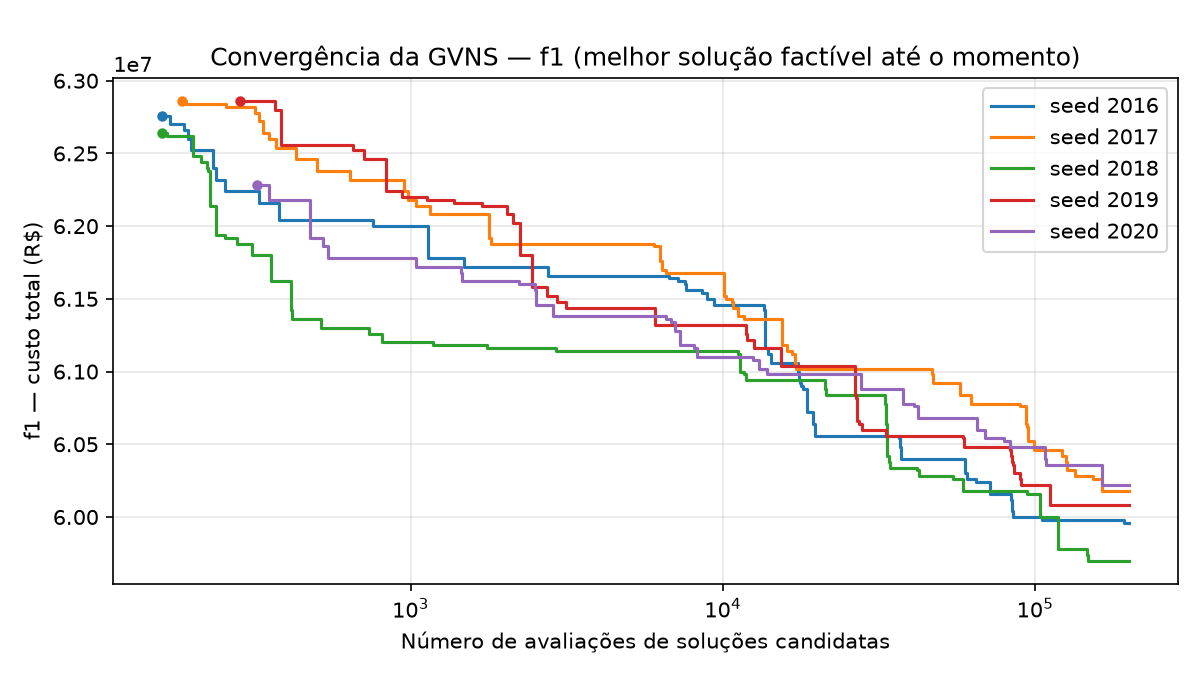
\includegraphics[width=\textwidth]{figures/convergence_f1.png}
        \caption{Otimização de $f_1$.}
    \end{subfigure}
    \hfill
    \begin{subfigure}[b]{0.32\textwidth}
        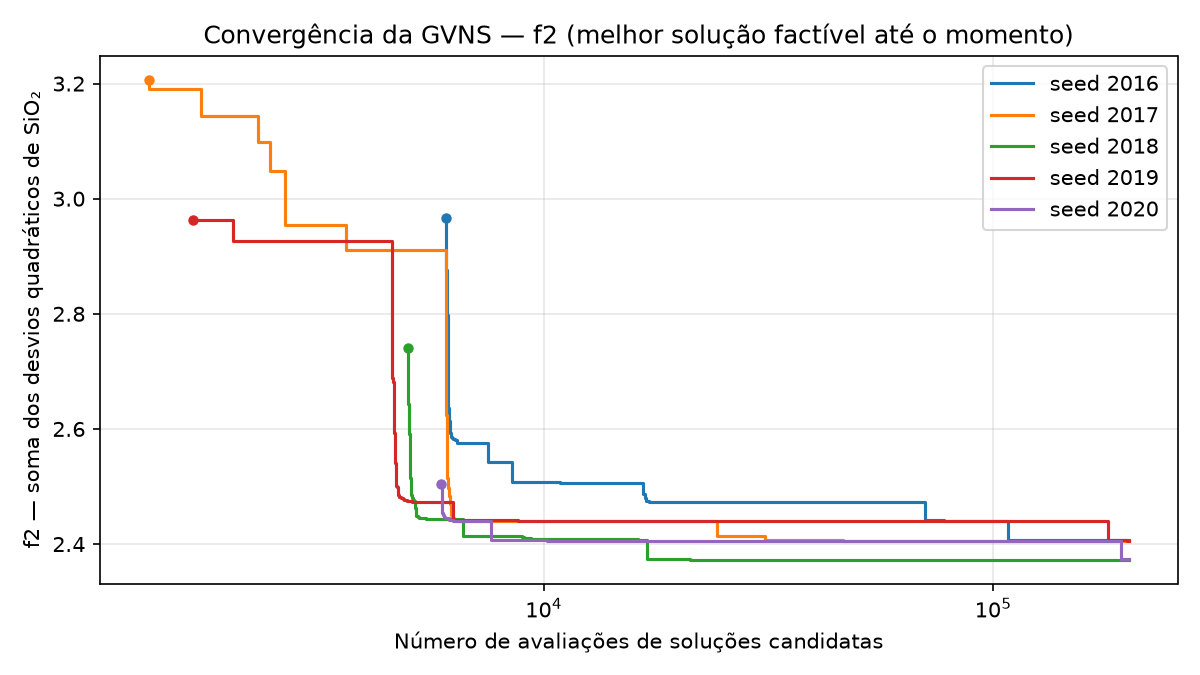
\includegraphics[width=\textwidth]{figures/convergence_f2.png}
        \caption{Otimização de $f_2$.}
    \end{subfigure}
    \hfill
    \begin{subfigure}[b]{0.32\textwidth}
        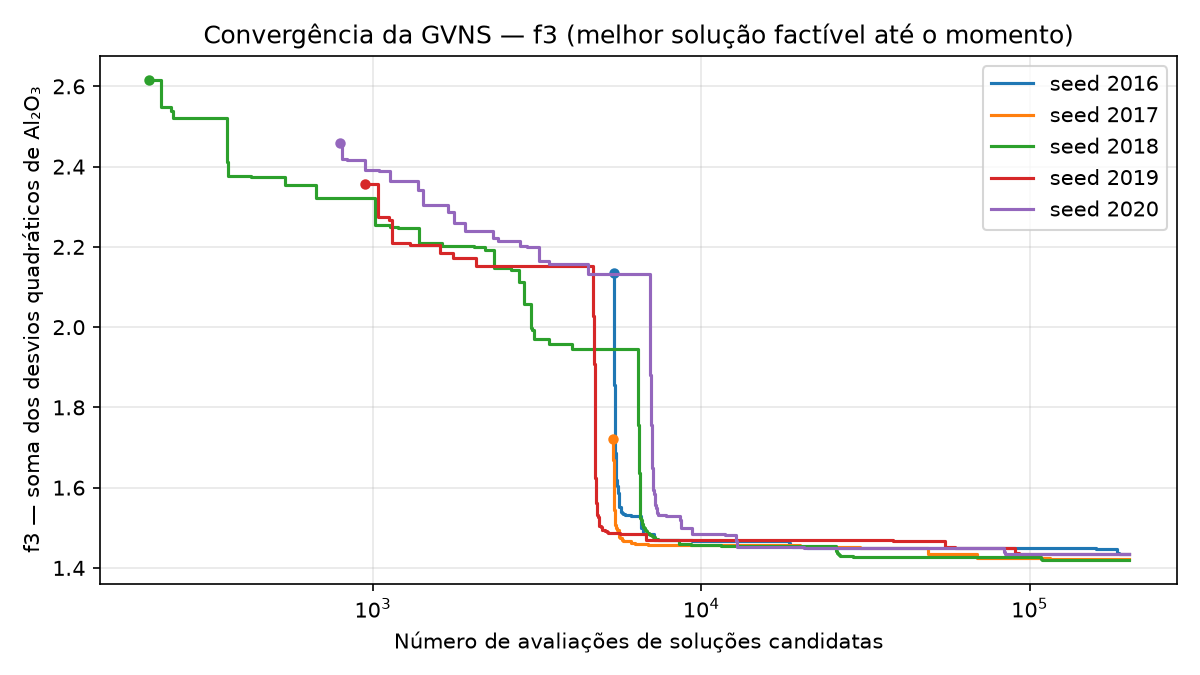
\includegraphics[width=\textwidth]{figures/convergence_f3.png}
        \caption{Otimização de $f_3$.}
    \end{subfigure}
    \caption{Curvas completas de convergência com as cinco execuções sobrepostas ao longo das avaliações de soluções candidatas (escala simétrica logarítmica). Os círculos marcam a primeira solução factível de cada execução.}
    \label{fig:curvas_convergencia}
\end{figure*}

\begin{figure*}[bp]
    \centering
    \begin{subfigure}[b]{0.32\textwidth}
        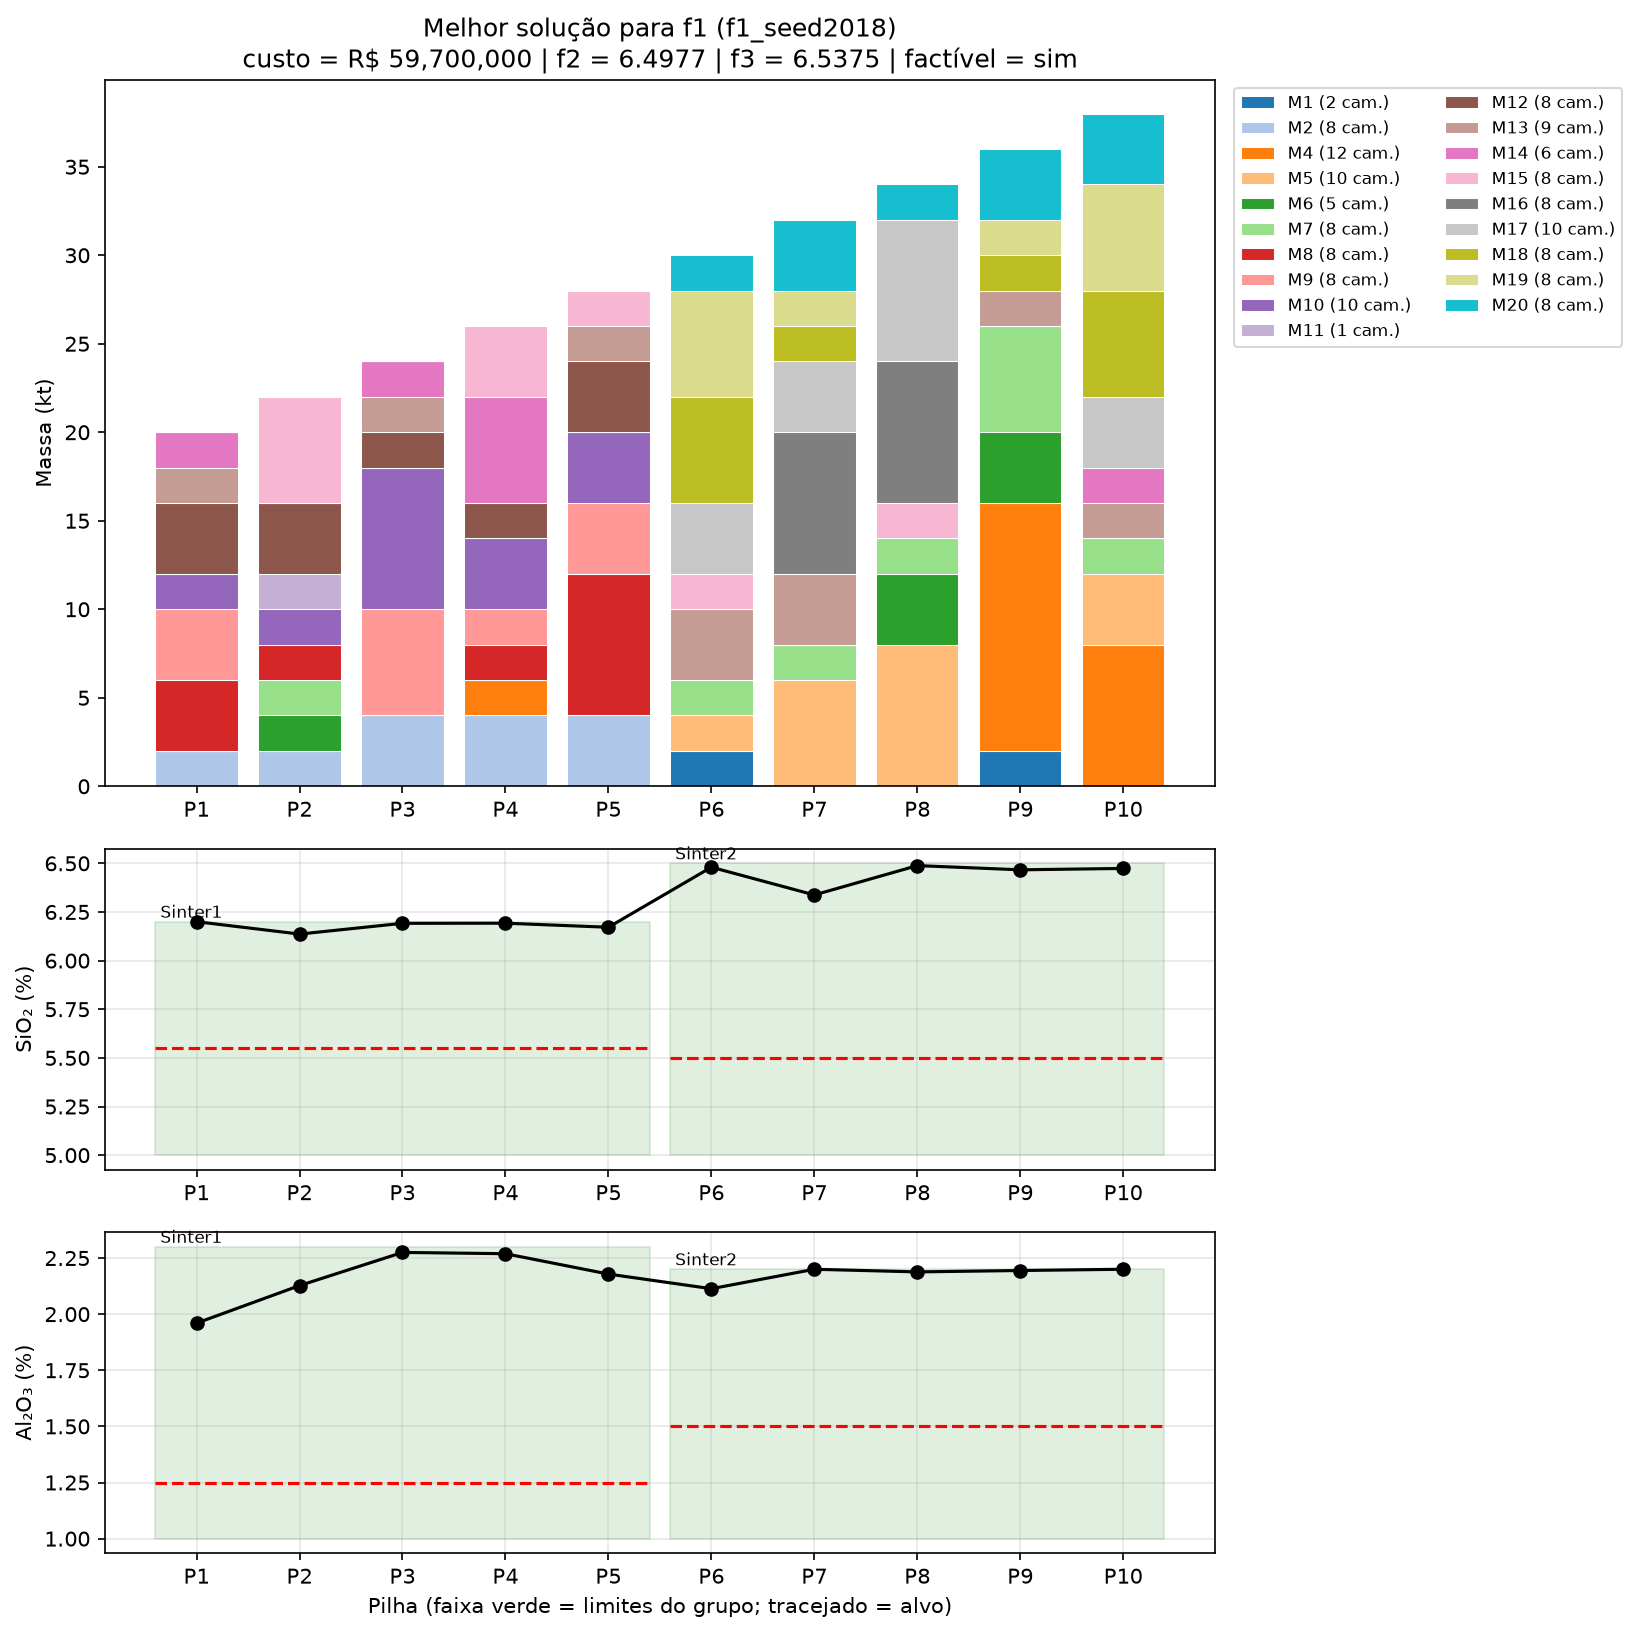
\includegraphics[width=\textwidth]{figures/best_solution_f1.png}
        \caption{Melhor solução de $f_1$ (seed 2018).}
    \end{subfigure}
    \hfill
    \begin{subfigure}[b]{0.32\textwidth}
        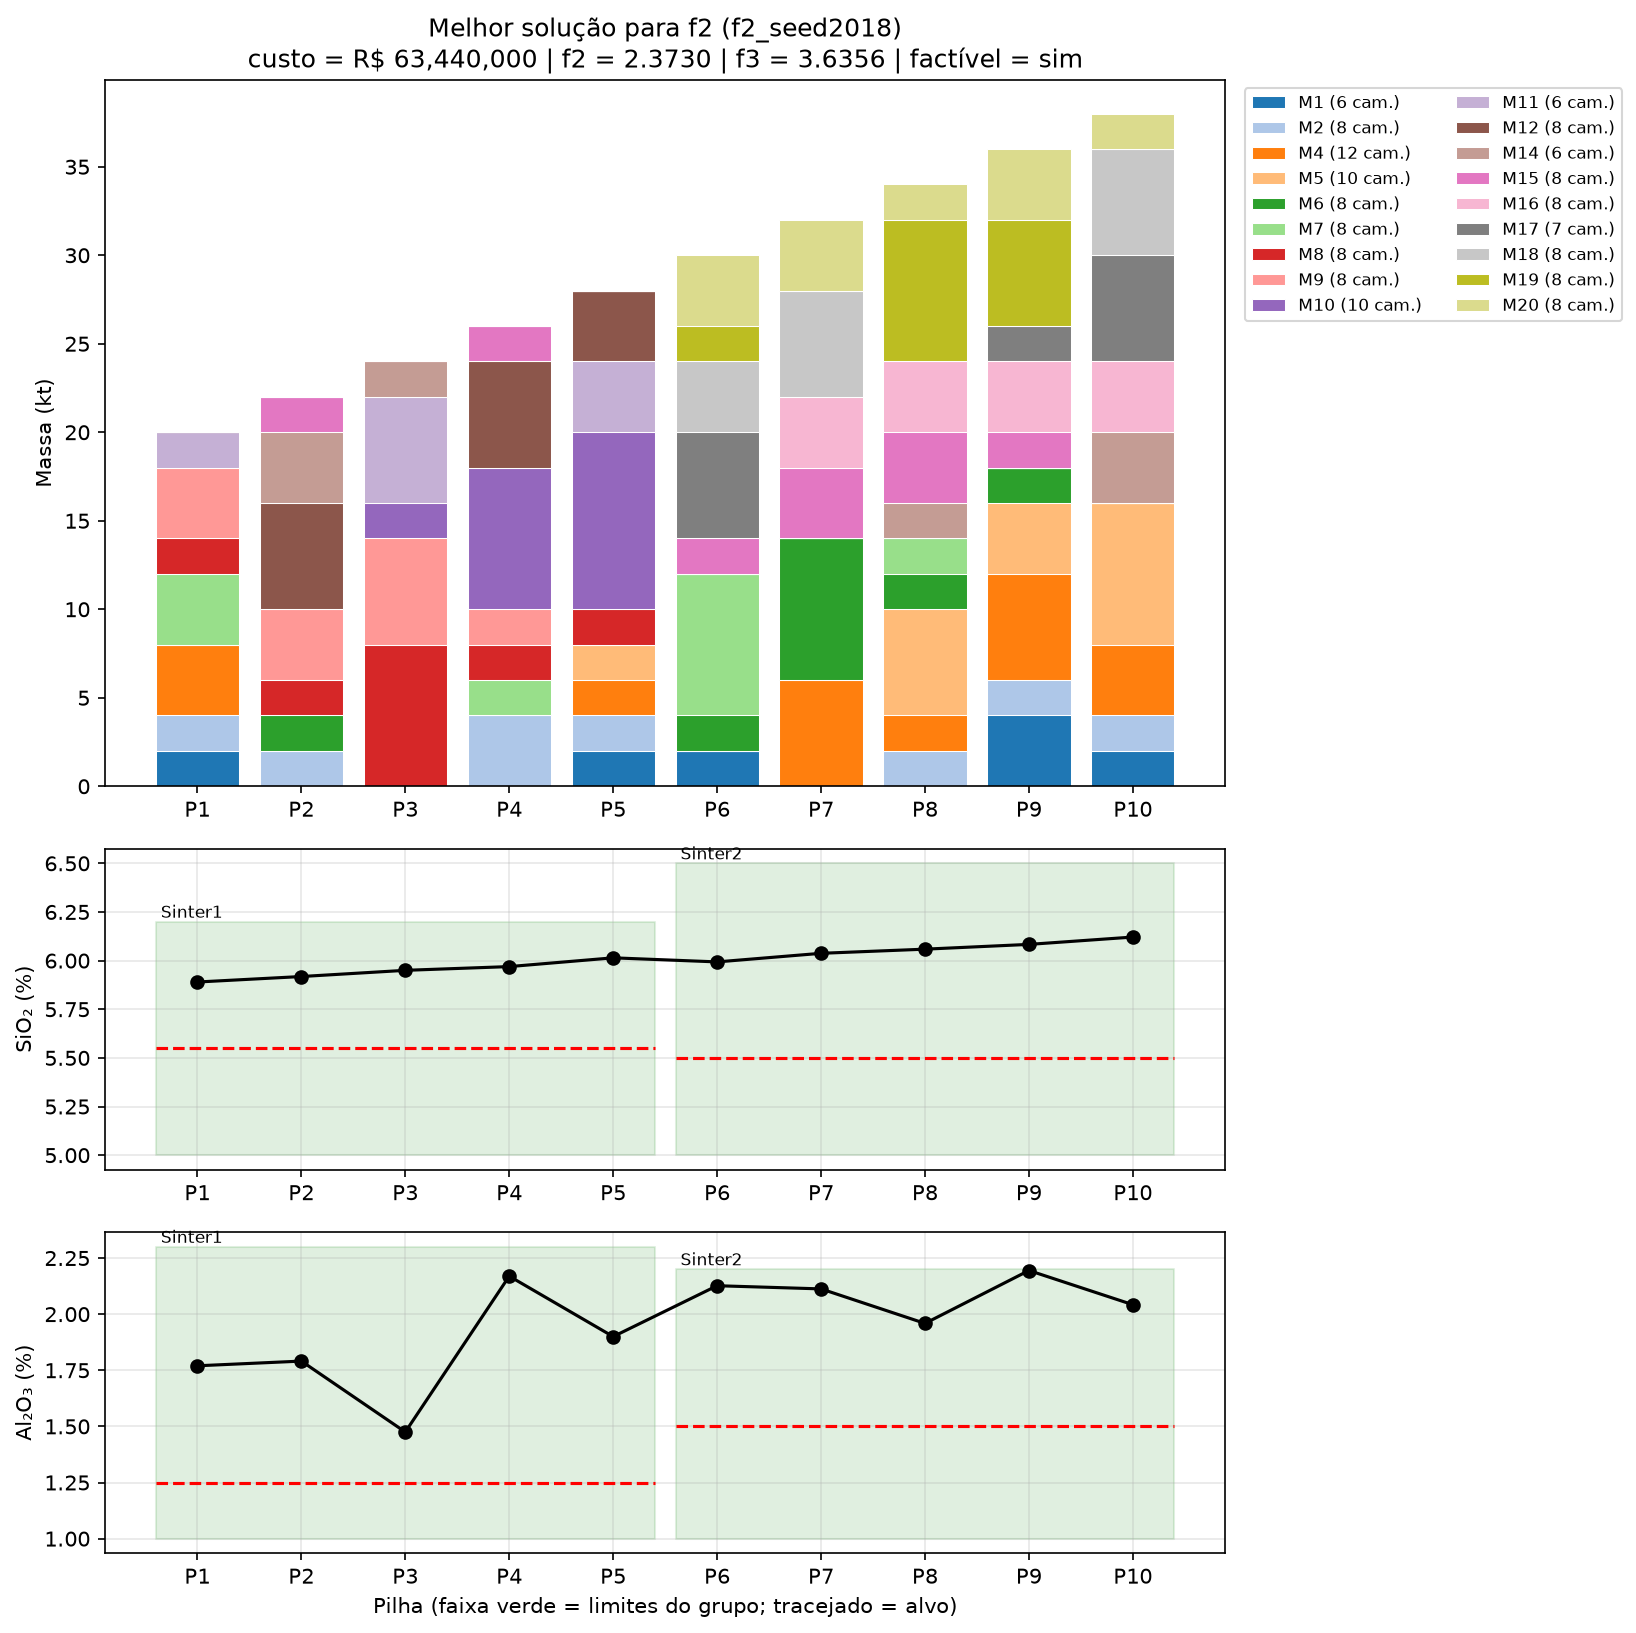
\includegraphics[width=\textwidth]{figures/best_solution_f2.png}
        \caption{Melhor solução de $f_2$ (seed 2018).}
    \end{subfigure}
    \hfill
    \begin{subfigure}[b]{0.32\textwidth}
        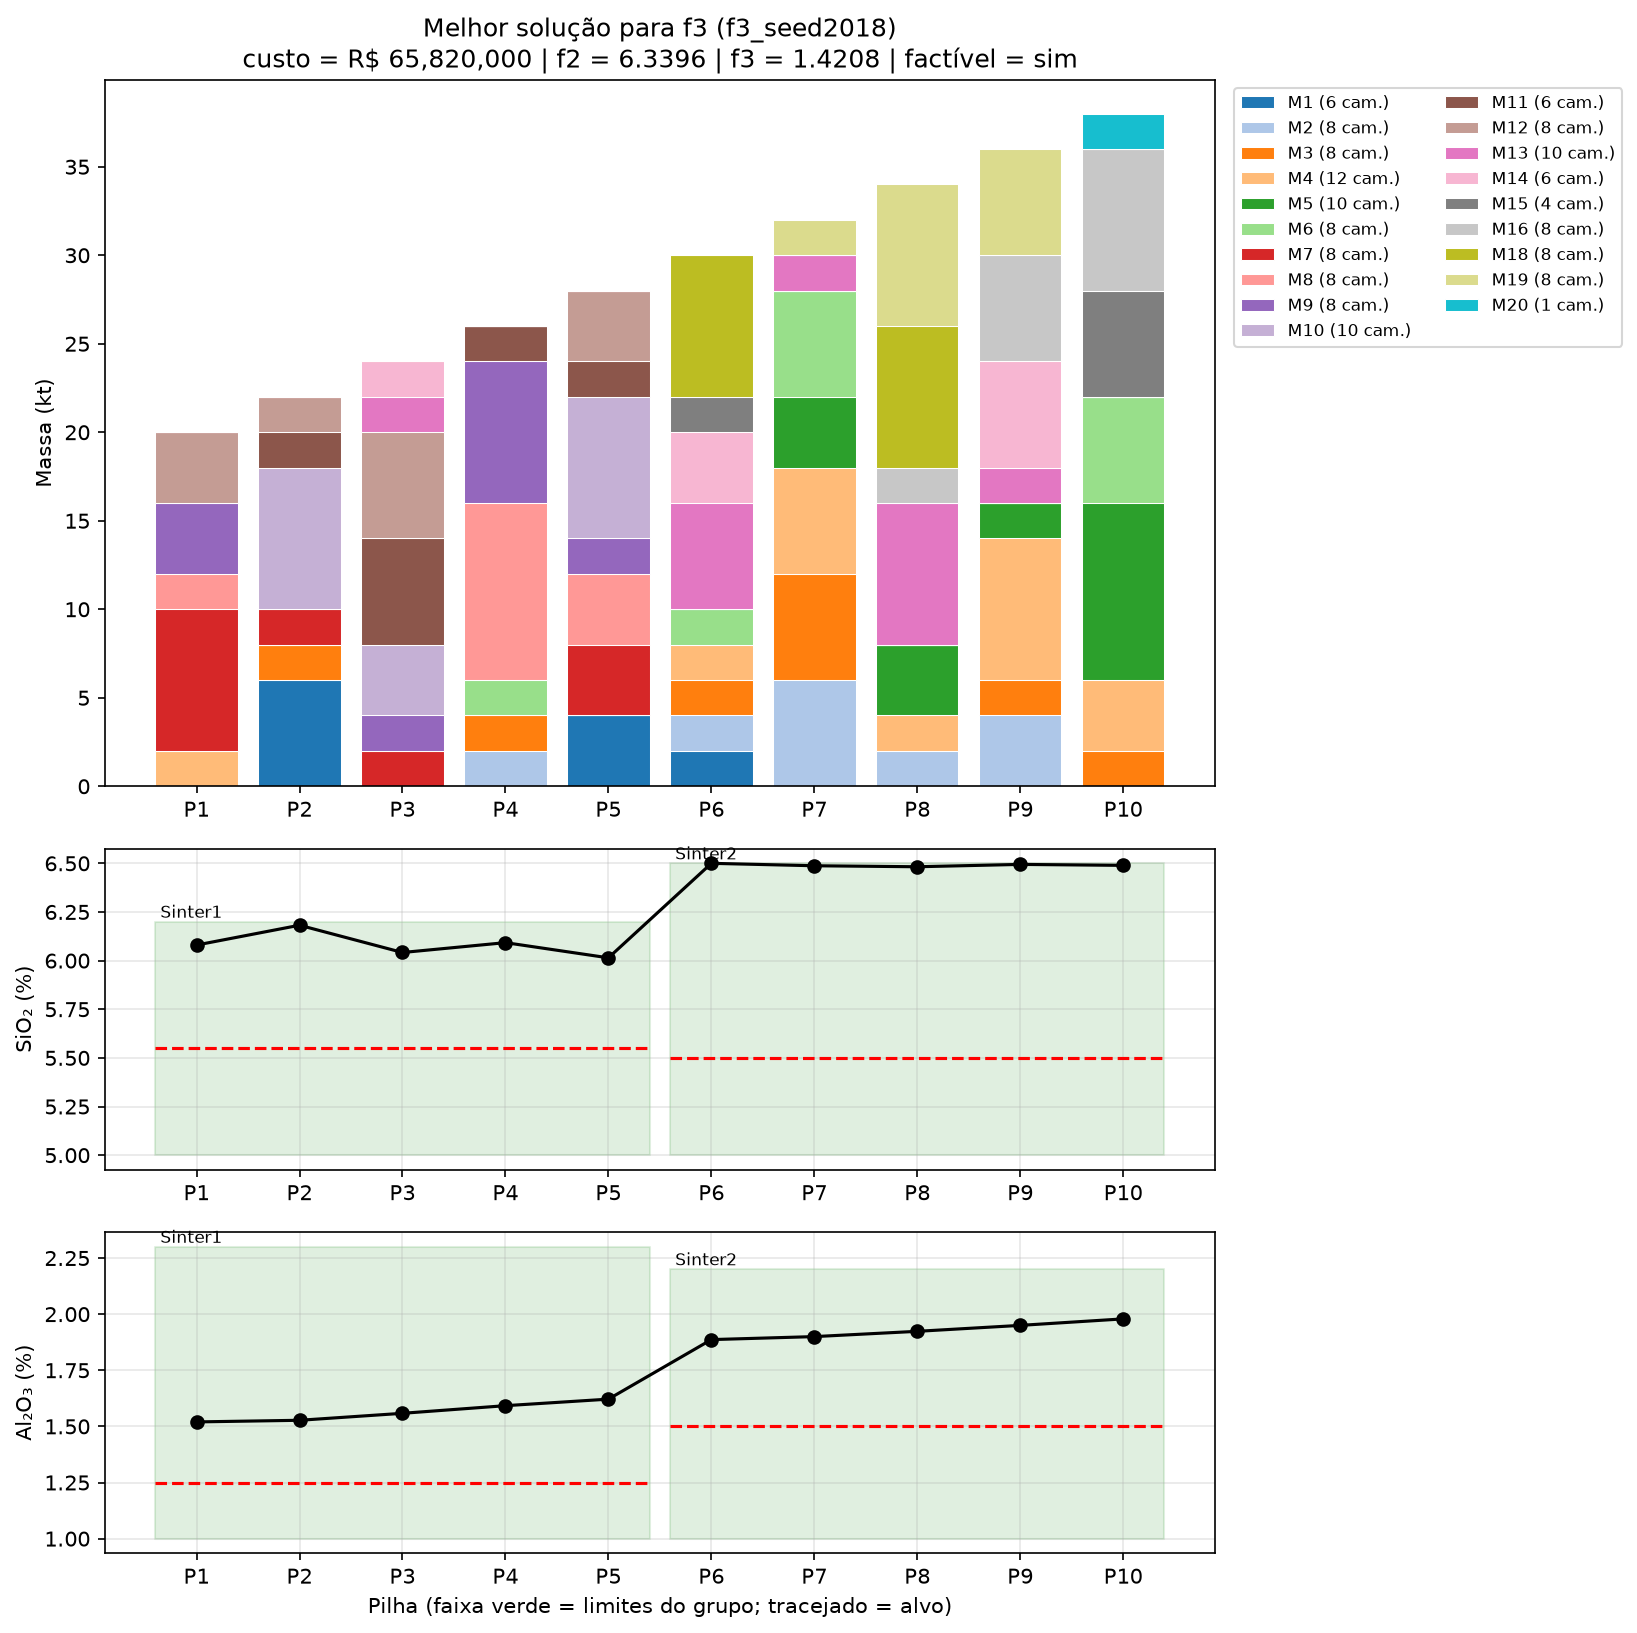
\includegraphics[width=\textwidth]{figures/best_solution_f3.png}
        \caption{Melhor solução de $f_3$ (seed 2018).}
    \end{subfigure}
    \caption{Representação completa das melhores soluções encontradas para cada objetivo: composição das pilhas por tipo de minério e massa (kt) no painel superior, e perfis de qualidade química de $\text{SiO}_2$ e $\text{Al}_2\text{O}_3$ frente às faixas admissíveis e alvos nos painéis inferiores.}
    \label{fig:melhores_solucoes}
\end{figure*}

As curvas da Fig.~\ref{fig:curvas_convergencia} mostram melhorias rápidas logo após a obtenção de factibilidade, seguidas por ganhos esparsos em horizontes maiores. Em $f_2$ e $f_3$, algumas seeds atingem patamares distintos por longos intervalos e voltam a melhorar após perturbações, o que justifica um orçamento suficientemente grande para permitir múltiplos ciclos de diversificação e intensificação.

\begin{table}[H]
\centering
\caption{Melhores soluções finais encontradas.}
\label{tab:melhores_solucoes}
\resizebox{\columnwidth}{!}{%
\begin{tabular}{lccccc}
\toprule
\textbf{Otimizado} & \textbf{seed} & \textbf{custo (R\$ mi)} & $f_2$ & $f_3$ & \textbf{primeira factível} \\
\midrule
$f_1$ & 2018 & 59,70 & 6,4977 & 6,5375 & 283 \\
$f_2$ & 2018 & 63,44 & 2,3730 & 3,6356 & 4.983 \\
$f_3$ & 2018 & 65,82 & 6,3396 & 1,4208 & 386 \\
\bottomrule
\end{tabular}%
}
\end{table}

A melhor solução de custo exige apenas R\$ 0,36 milhão a mais que a construtiva inicial barata e inviável, um acréscimo de aproximadamente 0,61\% para satisfazer todas as restrições. Entretanto, ela opera várias pilhas próximas aos limites superiores de qualidade: em Sinter 1, $\text{SiO}_2$ varia aproximadamente de 6,14\% a 6,20\%, e em Sinter 2 de 6,34\% a 6,49\%. Esse comportamento é coerente: em uma execução de $f_1$, aproximar-se do alvo químico não produz benefício adicional desde que as faixas admissíveis sejam respeitadas.

A otimização de $f_2$ reduziu o desvio de $\text{SiO}_2$ em aproximadamente 63,5\% em relação à melhor solução de custo, mas elevou o custo em 6,26\%. A otimização de $f_3$ reduziu o desvio de $\text{Al}_2\text{O}_3$ em aproximadamente 78,3\% e elevou o custo em 10,25\%. Esses números evidenciam o conflito que será tratado explicitamente na etapa multiobjetivo.

Mesmo nas execuções dedicadas a $f_2$ e $f_3$, os alvos não foram atingidos exatamente em todas as pilhas. Esse resultado não representa violação: alvo é um ponto desejado, enquanto os limites definem factibilidade. A composição é discreta, as disponibilidades são globais e a elegibilidade acopla as pilhas. Não foi produzida prova de ótimo global; portanto, os valores devem ser interpretados como os melhores encontrados pelo procedimento sob o orçamento fixado.

\section{Comportamento das vizinhanças}

As estatísticas internas permitem interpretar a função de cada operador. Em média, nas cinco execuções de $f_1$, $N_1$ produziu 775,2 melhorias locais, $N_2$ produziu zero e $N_3$ 1,6. O zero de $N_2$ é esperado, pois a troca preserva a quantidade global de cada minério e, consequentemente, o custo. Para $f_2$, as médias foram 256,0 melhorias $N_1$, 752,0 $N_2$ e 0,2 $N_3$; para $f_3$, 315,6 $N_1$, 995,4 $N_2$ e nenhuma $N_3$. Assim, $N_2$ é especialmente relevante para redistribuir qualidade entre pilhas sem alterar o uso global.

O baixo número de melhorias diretas de $N_3$ não implica inutilidade: ela amplia a topologia da busca local por um movimento coordenado que altera distribuição e composição global em um único passo. Além disso, a diversificação principal é realizada pelas estruturas $P_1$--$P_3$, separadas das vizinhanças locais. Em média, os níveis $P_1/P_2/P_3$ foram acionados 19,2/14,0/10,0 vezes em $f_1$, 12,2/9,6/7,8 em $f_2$ e 9,8/7,0/6,2 em $f_3$, mostrando que a busca alcançou repetidamente os níveis mais fortes quando perturbações menores não foram suficientes.

\section{Reprodutibilidade}

A execução final é reproduzida pelo comando abaixo a partir de uma versão limpa do código:
\begin{lstlisting}[language=bash]
python3 scripts/run_mono_experiments.py \
  --seeds 2016 2017 2018 2019 2020 \
  --budget 200000 \
  --sample-size 250 \
  --p1-positions 3 \
  --p2-chain-length 4 \
  --p3-piles 5 \
  --out results/mono_final
\end{lstlisting}

Cada arquivo JSON registra commit, instância, objetivo, seed, parâmetros, orçamento, tempo, viabilidade, composição e histórico best-so-far. O desvio-padrão apresentado é amostral ($n-1$). A separação entre seeds de calibração e seeds finais foi definida antes da rodada oficial.

\section{Conclusões}

Foi desenvolvida uma GVNS completa e reproduzível para as três versões mono-objetivo do problema de composição de pilhas. A representação por caminhões eliminou inviabilidades de massa e integralidade; elegibilidade foi preservada nos operadores; disponibilidade e qualidade foram tratadas por uma regra de viabilidade sem parâmetro de penalização. A VND combinou $N_1$ completa com $N_2/N_3$ amostradas, enquanto $P_1$--$P_3$ forneceram níveis independentes de perturbação.

A calibração em etapas permitiu consolidar uma configuração única para os três objetivos: amostra 250, SHAKE 3/4/5 e orçamento de 200.000 avaliações. Todas as 15 execuções finais foram factíveis, com baixa dispersão entre seeds. Os resultados mostram que soluções de menor custo tendem a operar mais próximas das fronteiras de qualidade, enquanto reduções de desvio químico requerem custos maiores. Essa evidência é o principal insumo para a Entrega 2, na qual os três objetivos serão tratados conjuntamente por técnicas multiobjetivo e normalização baseada nas referências mono-objetivo obtidas aqui.

{\small
\begin{thebibliography}{9}

\bibitem{case_enunciado}
Universidade Federal de Minas Gerais. \textit{Teoria da Decisão -- Case: Otimização do Custo e Qualidade de Pilhas de Minério}. Enunciado da disciplina, 2026/2.

\bibitem{aulas_td}
Universidade Federal de Minas Gerais. \textit{Material de aula de Teoria da Decisão: VNS/GVNS e tratamento de restrições}. 2026/2.

\bibitem{repo_projeto}
Grupo do projeto. \textit{cassotis\_optimization}. Repositório GitHub com o código das execuções finais. 2026.

\end{thebibliography}
}

\end{document}
